\usetikzlibrary{arrows.meta,calc}
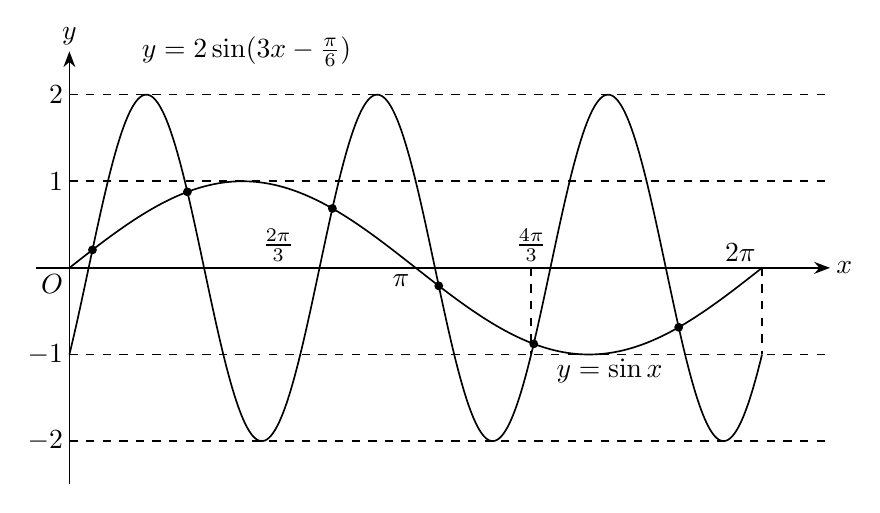
\begin{tikzpicture}[x=1.4cm,y=1.1cm,line width=.6pt,>=Stealth,font=\normalsize]
% axes beyond 2pi by half step
\draw[->] (-0.3,0)--(6.9,0) node[right,inner sep=0pt,xshift=2pt] {$x$};
\draw[->] (0,-2.5)--(0,2.5) node[above,inner sep=0pt,yshift=2pt] {$y$};
\node[below left,inner sep=0pt,xshift=-2pt,yshift=-2pt] at (0,0) {$O$};
% dashed helpers y=+-1,+-2
\draw[dashed] (0,2)--(6.9,2);
\draw[dashed] (0,1)--(6.9,1);
\draw[dashed] (0,-1)--(6.9,-1);
\draw[dashed] (0,-2)--(6.9,-2);
% vertical helpers at 4pi/3 and 2pi
\draw[dashed] (4.1887902,0)--(4.1887902,-1);
\draw[dashed] (6.2831853,0)--(6.2831853,-1);
% exact curves
\draw[domain=0:6.2831853,samples=220] plot (\x,{sin(deg(\x))});
\draw[domain=0:6.2831853,samples=400] plot (\x,{2*sin(3*deg(\x)-30)});
% six intersection dots (bisection values, verified in construction.py)
\fill (0.2092,0.2077) circle (1.6pt);
\fill (1.0704,0.8774) circle (1.6pt);
\fill (2.3856,0.6860) circle (1.6pt);
\fill (3.3508,-0.2077) circle (1.6pt);
\fill (4.2119,-0.8774) circle (1.6pt);
\fill (5.5272,-0.6860) circle (1.6pt);
% x ticks
\node[above left,inner sep=0pt,xshift=-2pt,yshift=2pt] at (2.0943951,0) {$\frac{2\pi}{3}$};
\node[below left,inner sep=0pt,xshift=-2pt,yshift=-2pt] at (3.1415927,0) {$\pi$};
\node[above,inner sep=0pt,xshift=0pt,yshift=2pt] at (4.1887902,0) {$\frac{4\pi}{3}$};
\node[above left,inner sep=0pt,xshift=-2pt,yshift=2pt] at (6.2831853,0) {$2\pi$};
% y ticks
\node[left,inner sep=0pt,xshift=-2pt] at (0,2) {$2$};
\node[left,inner sep=0pt,xshift=-2pt] at (0,1) {$1$};
\node[left,inner sep=0pt,xshift=-2pt] at (0,-1) {$-1$};
\node[left,inner sep=0pt,xshift=-2pt] at (0,-2) {$-2$};
% curve labels in whitespace with clearance
\node[above right,inner sep=0pt,xshift=2pt,yshift=2pt] at (0.6,2.25) {$y=2\sin(3x-\frac{\pi}{6})$};
\node[below,inner sep=0pt,xshift=0pt,yshift=-2pt] at (4.9,-0.9824526126) {$y=\sin x$};
\end{tikzpicture}
